% Created 2017-11-07 Tue 07:42
\documentclass[11pt]{article}
\usepackage[utf8]{inputenc}
\usepackage[T1]{fontenc}
\usepackage{fixltx2e}
\usepackage{graphicx}
\usepackage{longtable}
\usepackage{float}
\usepackage{wrapfig}
\usepackage{rotating}
\usepackage[normalem]{ulem}
\usepackage{amsmath}
\usepackage{textcomp}
\usepackage{marvosym}
\usepackage{wasysym}
\usepackage{amssymb}
\usepackage{hyperref}
\tolerance=1000
\usepackage{minted}
\usepackage{fancyhdr}
\setcounter{secnumdepth}{-1} 
\pagestyle{fancy}
\fancyhead{} 
\rhead{\textit{Michael Laufer}}
\lhead{\textit{Numerical Methods Fall 2017, HW6}}
\small

\author{Michael Laufer}
\date{\today}
\title{HW1 Numerical Methods Fall 2017}
\hypersetup{
  pdfkeywords={},
  pdfsubject={},
  pdfcreator={Emacs 25.3.1 (Org mode 8.2.10)}}
\begin{document}

\maketitle
\section{1.1 Elliptic, Parabolic, Hyperbolic PDEs}
\label{sec-1}
\subsection{\textbf{a.}}
\label{sec-1-1}
\[
\frac{\partial \phi}{\partial t} + \vec{U} \cdot \nabla \phi = 0
\]
There are no second order derivatives, therefore $b^{2} -4ac = 0$         . The PDE is parabolic.
\subsection{\textbf{b.}}
\label{sec-1-2}
\[
\frac{\partial \phi}{\partial t} + \vec{U} \cdot \nabla \phi = \Gamma \nabla^{2} \phi
\]
We can see that \$ a=c=-$\Gamma$ \$ where $\Gamma$ is a positive number. Therefore $b^{2} -4ac < 0$. The PDE is elliptic.

\subsection{\textbf{c.}}
\label{sec-1-3}
\[
\frac{\partial}{\partial x}  \left[ \Gamma_{1} \frac{\partial}{\partial x} -\Gamma_{2} \frac{\partial}{\partial y} \right]  + \frac{\partial}{\partial y}  \left[ \Gamma_{1} \frac{\partial}{\partial y} -\Gamma_{2} \frac{\partial}{\partial x} \right] = 0
\]
Rearranging the equation:
\[
 \Gamma_{1} \frac{\partial^{2} \phi}{\partial x^{2}} - 2 \Gamma_{2}  \frac{\partial^{2} \phi}{\partial x \partial y} + \Gamma_{1} \frac{\partial^{2} \phi^}{\partial y^{2}} = 0
\]
$\Gamma_{1}$ and $\Gamma_{2}$ can be either positive or negative.
Splitting into different cases:
\begin{itemize}
\item If $\Gamma_{1} > \Gamma_{2}$: $b^{2} -4ac > 0$ and the PDE is hyperbolic
\item If $\Gamma_{1} < \Gamma_{2}$: $b^{2} -4ac < 0$ and the PDE is elliptic
\item If $\Gamma_{1} = \Gamma_{2}$: $b^{2} -4ac = 0$ and the PDE is parabolic.
\end{itemize}
\subsection{\textbf{d.}}
\label{sec-1-4}
\[
\frac{\partial \phi}{\partial t} - \frac{1}{r}\frac{\partial}{\partial r}\left( r \frac{\phi}{\partial r} \right) = 0
\]
Rearranging the equation:
\[
\frac{\partial \phi}{\partial t} - \frac{1}{r}\frac{\partial \phi}{\partial r} - \frac{\partial^{2} \phi}{\partial r^{2}} = 0
\]
$b^{2} -4ac = 0$. The PDE is parabolic.

\subsection{\textbf{e.}}
\label{sec-1-5}
\[
\frac{\partial^{2} \phi}{\partial t^{2}} + \frac{\partial \phi}{\partial t} - \nabla \cdot \left(\Gamma \nabla \phi \right) = \phi
\]
Rearranging yields,
\[
\frac{\partial^{2} \phi}{\partial t^{2}} + \frac{\partial \phi}{\partial t} - \Gamma \nabla^{2} \phi - \phi = 0
\]
In regards to space, the PDE is clearly elliptic as only a single second order spatial derivative exists. In regards to a time-space point of view, given $\Gamma > 0$,  $b^{2} -4ac > 0$. The PDE is hyperbolic.
\newpage

\section{1.2 Galerkin FE method}
\label{sec-2}
Given: 
\[
\frac{\partial^{2} \phi}{\partial x^{2}} = \cos x
\]
With the boundary conditions:
\[
 \phi \left( 0 \right) = 0, \phi \left( 1 \right) = 1, 
\]
The analytical solution is found by integrating twice with respect to $\phi$ and plugging in the provided boundary conditions, resulting in:
\[
\phi(x) = -\cos(x) +  \cos(1) x +1
\]
To solve this equation using the Galerkin Finite Element method we will follow the same procedure as Example 1.1, and choose the same top-hat linear base functions but with a different right hand side.\\
Using the same basis function gives us the same interior tradiagonal stiffness values: \\
if $i=j$, $K_{j,i} = 2 / \Delta x$ \\
if $i = j+1$ or $i = j-1$, $K_{j,i} = -1 / \Delta x$ \\
The interior node load vector values are computed just as in example 1.1. Utilizing integration by parts leads to:
\[
F_{j}=-\int_{0}^{1} \cos x \psi(x)dx = \frac{-1}{\Delta x} \left(\int_{x_{i-1}}^{x_{i}} \cos x \left(x -x_{i-1} \right)dx + \int_{x_{i}}^{x_{i+1}} \cos x \left(x_{i+1} -x \right)dx \right) =
\]
\[
= \frac{-1}{\Delta x} \left( 2\cos x_{i}  - \cos x_{i-1}  - \cos x_{i+1}\right)
\] 
which is valid for $2 \leq j \leq n-1$

Regarding boundary conditions, we first notice that the we can infer that $a_{1}=0$ and $a_{n}=1$.
In order to take these values into account in our system, we will force the values at the boundary nodes, leading to the equation: 

\[
K_{j,i}a_{i}=F_{j}
\]

Or more explicitly written: \\
\begin{bmatrix}
 1 &  0 & 0 & 0 & 0 \\-1/dx & 2/dx & -1/dx &0 &0 \\ 0& -1/dx & 2/dx & -1/dx &0 \\ 0& 0& -1/dx & 2/dx & -1/dx \\ 0 & 0 & 0 & 0 & 1  
\end{bmatrix} 
\begin{bmatrix} 
a_{1} \\ a_{2} \\ a_{3} \\ a_{4} \\ a_{5} &  \end{bmatrix}
=
\begin{bmatrix}
 0 \\ F_{2} \\ F_{3} \\ F_{4} \\ 1  
\end{bmatrix} 

\newpage

Due to fact the matrix is banded (in this case tridiagonal), we can employ the Scipy banded solver, which solves banded matrices much faster and more efficiently than the Numpy linear algebra solver.

\begin{minted}[]{python}
from scipy.linalg import solve_banded
def tridiagsolver(K,F)
    ud = np.insert(np.diag(K,1), 0, 0)           # upper diagonal
    d = np.diag(K)                               # main diagonal
    ld = np.insert(np.diag(K,-1), len(F)-1, 0)   # lower diagonal
    ab = np.matrix([ud, d, ld])                  # simplified matrix
    a = solve_banded((1, 1), ab, F)
    return a
\end{minted}

A plot of the numerical solution plotted against the analytical solution can be seen here for both a 5 node system as well as a 9 node system:
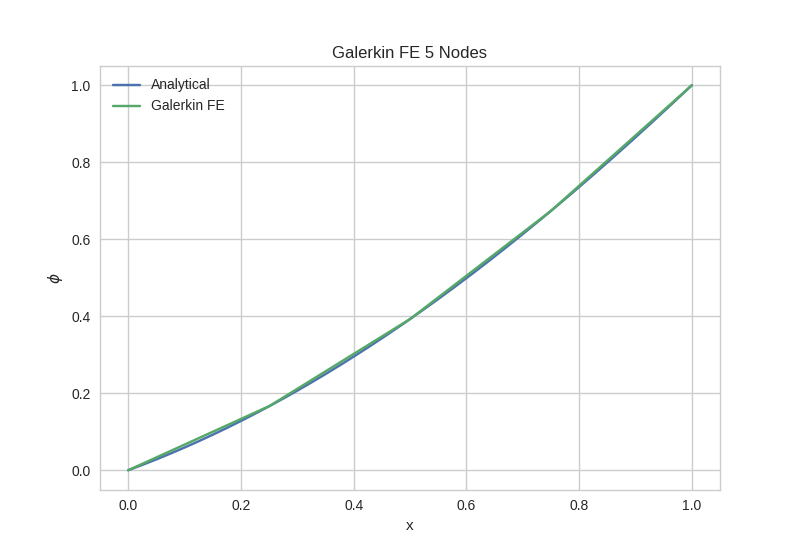
\includegraphics[width=12cm]{./figures/5nodes.png}

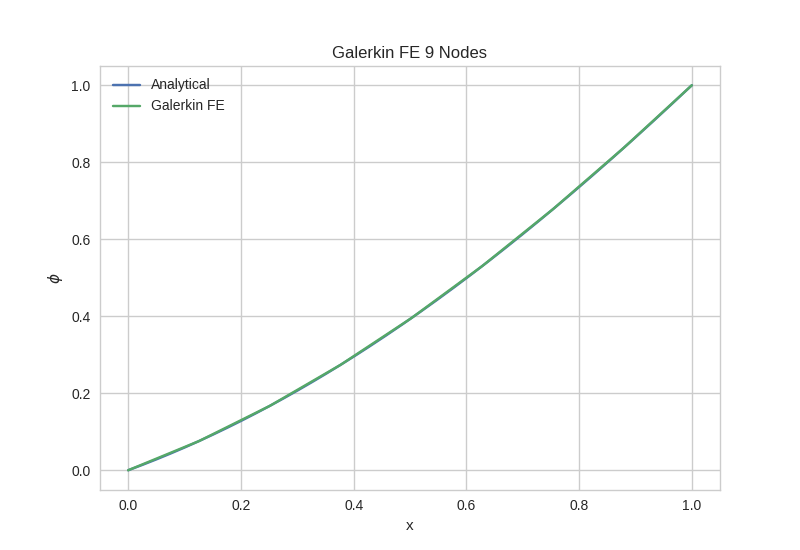
\includegraphics[width=12cm]{./figures/9nodes.png}

We can see that even for 5 nodes, an accurate solution is obtained.
Additionally a plot of the error throughout the domain can be plotted.

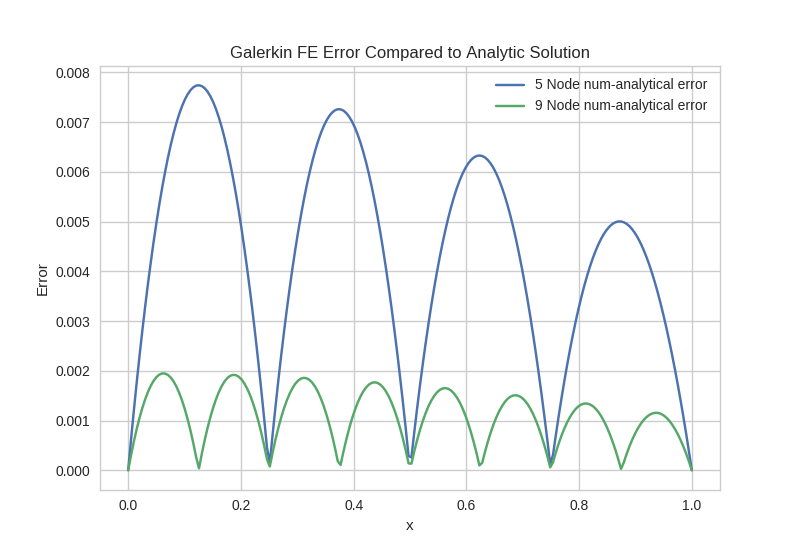
\includegraphics[width=12cm]{./figures/error.png}

We can see that at nodal values we get particularly good accuracy. We can also observe that errors are largest as the point moves away from the nodal points.

The fluxes are computed by differentiating the $\phi (x)$ expansion. The coefficients are constant with regard to the spatial derivative and thus:
\[
J_{L} = \frac{\partial \phi}{\partial x} (0) = a_{1} \frac{-1}{dx} + a_{2} \frac{1}{dx}  
\]

\[
J_{R} = \frac{\partial \phi}{\partial x} (1) = a_{n} \frac{1}{dx} + a_{n-1} \frac{-1}{dx} 
\]

Lastly the net source in the domain by integration is computed by integrating the source term analytically from 0 to 1:
\[
S = \int_{0}^{1} \cos x
\] 

Numerical results are compared with analytical results in the following table:\\

\begin{center}
\begin{tabular}{|c|c|c|c|}
\hline
 & \textbf{Analytical} & \textbf{Galerkin FE 5 Nodes} & \textbf{Galerkin FE 9 Nodes}\\
\hline
$J_{L}$ & 0.5403 & 0.66464 & 0.60272\\
$J_{R}$ & 1.3817 & 1.3058 & 1.3458\\
$S$ & 0.8414 & - & -\\
$I= J_{R}-J_{L}-S$ & 0 & -0.202 & -0.0983\\
\hline
\end{tabular}
\end{center}
It is clear that as more nodes are added, the solution better converges to the analytical solution.
We can observe that $I \neq 0$ for the numerical cases, indicating that the local conservation is not satisfied.    
This is a clear  disadvantage of the Galerkin FE method compared to Finite Volume methods that in general satisfy conservation.

\newpage
\subsection{Appendix: Python Code}
\label{sec-2-1}
\begin{minted}[]{python}
import numpy as np
import matplotlib.pyplot as plt
from scipy.linalg import solve_banded
import math
import seaborn as sns
sns.set_style("whitegrid")


def tridiagsolver(K,F):
    ud = np.insert(np.diag(K,1), 0, 0)           # upper diagonal
    d = np.diag(K)                               # main diagonal
    ld = np.insert(np.diag(K,-1), len(F)-1, 0)   # lower diagonal
    ab = np.matrix([ud, d, ld])                  # simplified matrix
    a = solve_banded((1, 1), ab, F)
    return a

def psi(j,x, dx):
    if x > (j+1)*dx or x < (j-1)*dx:
	return 0
    elif x < j*dx:
	return (x - (j-1)*dx)/dx
    else:
	return ((j+1)*dx - x)/dx

def galerkin1d(nx):
    x = np.linspace(0,1,nx)
    dx = 1.0/(nx-1)
    K = np.zeros((nx,nx))                   # Stiffness matrix
    for i in range(nx):
	if i == 0:
	    K[i,i] = 1
	    K[i,i+1] = 0
	elif i == len(K)-1:
	    K[i,i] = 1
	    K[i,i-1] = 0
	else:
	    K[i,i] = 2/dx
	    K[i,i-1] = -1/dx
	    K[i,i+1] = -1/dx

    F = np.zeros(nx)                         # Load vector
    F [0] = 0
    F[1:-1] = (-1.0/dx)*(2*np.cos(x[1:-1]) - np.cos(x[0:-2]) - np.cos(x[2:]))
    F[-1] = 1

    a = tridiagsolver(K,F)                   # Solve system

    nxplot = 200                             # Recombine phi from basis functions
    plot_x = np.linspace(0,1,nxplot)
    phi_galerkin = np.zeros(nxplot)
    for i in range(len(plot_x)):                    
	for j in range(len(a)):
	    phi_galerkin[i] +=  a[j]*psi(j, plot_x[i], dx)
    return phi_galerkin

if __name__ == "__main__":
    plot_x = np.linspace(0,1,200)  
    phi_galerkin5 = galerkin1d(nx=5)
    phi_galerkin9 = galerkin1d(nx=9)
    phi_analy = -np.cos(plot_x) + np.cos(1)*plot_x + 1

    plt.figure(1)
    plt.plot(plot_x, phi_analy, label= "Analytical")
    plt.plot(plot_x, phi_galerkin5, label="Galerkin FE")
    plt.title("Galerkin FE 5 Nodes")
    plt.ylabel("$\phi$")
    plt.xlabel("x")
    plt.legend()

    plt.figure(2)
    plt.plot(plot_x, phi_analy, label= "Analytical")
    plt.plot(plot_x, phi_galerkin9, label="Galerkin FE")
    plt.title("Galerkin FE 9 Nodes")
    plt.ylabel("$\phi$")
    plt.xlabel("x")
    plt.legend()

    plt.figure(3)
    plt.plot(plot_x, np.abs(phi_analy-phi_galerkin5), label= "5 Node num-analytical error")
    plt.plot(plot_x, np.abs(phi_analy-phi_galerkin9), label= "9 Node num-analytical error")
    plt.title("Galerkin FE Error Compared to Analytical Solution")
    plt.ylabel("Error")
    plt.xlabel("x")
    plt.legend()
    plt.show()
\end{minted}
% Emacs 25.3.1 (Org mode 8.2.10)
\end{document}